\documentclass[12pt,a4paper,openany]{book}

% ===== PACKAGES =====
\usepackage[utf8]{inputenc}
\usepackage[T1]{fontenc}
\usepackage{microtype}
\usepackage{amsmath,amssymb,amsthm}
\usepackage{graphicx}
\usepackage{xcolor}
\usepackage{tikz}
\usepackage{listings}
\usepackage{hyperref}
\usepackage{booktabs}
\usepackage{enumitem}
\usepackage{fancyhdr}
\usepackage{titlesec}
\usepackage{tcolorbox}
\usepackage{fontawesome5}
\usepackage{mdframed}
\usepackage{subcaption}
\usepackage{wrapfig}
\usepackage{gensymb}

% ===== GEOMETRY - SMALLER MARGINS =====
\usepackage[
    top=3cm,
    bottom=3cm,
    left=3cm,
    right=3cm,
    marginparwidth=1.8cm,
    marginparsep=0.3cm,
    headheight=15pt,
    headsep=1cm,
    footskip=1cm
]{geometry}

% ===== COLORS =====
\definecolor{noteblue}{RGB}{13, 110, 253}
\definecolor{tipgreen}{RGB}{25, 135, 84}
\definecolor{importantorange}{RGB}{255, 149, 0}
\definecolor{warningyellow}{RGB}{255, 193, 7}
\definecolor{cautionred}{RGB}{220, 53, 69}
\definecolor{codegray}{RGB}{248, 249, 250}
\definecolor{linkblue}{RGB}{0, 123, 255}

% ===== HYPERREF SETUP =====
\hypersetup{
    colorlinks=true,
    linkcolor=linkblue,
    citecolor=linkblue,
    urlcolor=linkblue,
    bookmarksdepth=3,
    pdfborder={0 0 0}
}

% ===== GITHUB-STYLE CALLOUT BOXES =====
\tcbuselibrary{skins,breakable}

% Base style for all callouts - GitHub-like design
\tcbset{
    calloutbase/.style={
        enhanced,
        breakable,
        sharp corners,
        colback=white,
        colframe=#1,
        borderline west={3pt}{0pt}{#1},
        boxrule=1pt,
        left=12pt,
        right=8pt,
        top=8pt,
        bottom=8pt,
        fonttitle=\bfseries\sffamily\small,
        coltitle=#1,
        title style={left color=#1!10, right color=#1!5},
        before skip=1.5\baselineskip,
        after skip=1.5\baselineskip,
    }
}

% NOTE callout - Blue theme
\newtcolorbox{noteblock}{
    calloutbase=noteblue,
    colback=noteblue!3,
    title={\textcolor{noteblue}{\faInfoCircle}\ \textcolor{noteblue}{NOTE}}
}

% TIP callout - Green theme  
\newtcolorbox{tipblock}{
    calloutbase=tipgreen,
    colback=tipgreen!3,
    title={\textcolor{tipgreen}{\faLightbulb}\ \textcolor{tipgreen}{TIP}}
}

% IMPORTANT callout - Orange theme
\newtcolorbox{importantblock}{
    calloutbase=importantorange,
    colback=importantorange!3,
    title={\textcolor{importantorange}{\faExclamationCircle}\ \textcolor{importantorange}{IMPORTANT}}
}

% WARNING callout - Yellow theme
\newtcolorbox{warningblock}{
    calloutbase=warningyellow,
    colback=warningyellow!3,
    title={\textcolor{warningyellow!80!black}{\faExclamationTriangle}\ \textcolor{warningyellow!80!black}{WARNING}}
}

% CAUTION callout - Red theme
\newtcolorbox{cautionblock}{
    calloutbase=cautionred,
    colback=cautionred!3,
    title={\textcolor{cautionred}{\faExclamationTriangle}\ \textcolor{cautionred}{CAUTION}}
}
% ===== CODE LISTINGS - C LANGUAGE =====
\lstset{
    backgroundcolor=\color{codegray},
    basicstyle=\ttfamily\footnotesize,
    breakatwhitespace=false,
    breaklines=true,
    captionpos=b,
    commentstyle=\color{gray},
    frame=single,
    frameround=tttt,
    framesep=5pt,
    keywordstyle=\color{blue},
    language=C,
    numbers=left,
    numbersep=5pt,
    numberstyle=\tiny\color{gray},
    rulecolor=\color{black},
    showspaces=false,
    showstringspaces=false,
    showtabs=false,
    stringstyle=\color{red},
    tabsize=4,
    morekeywords={size_t, ssize_t, socklen_t, struct, typedef}
}

% ===== CHAPTER AND SECTION FORMATTING =====
\titleformat{\chapter}[display]
  {\normalfont\huge\bfseries\sffamily}
  {\chaptertitlename\ \thechapter}
  {20pt}
  {\Huge}
  
\titleformat{\section}
  {\normalfont\Large\bfseries\sffamily}
  {\thesection}
  {1em}
  {}
  
\titleformat{\subsection}
  {\normalfont\large\bfseries\sffamily}
  {\thesubsection}
  {1em}
  {}

% ===== HEADER AND FOOTER =====
\pagestyle{fancy}
\fancyhf{}
\fancyhead[LE]{\small\sffamily\color{darkblue}\nouppercase{\leftmark}}
\fancyhead[RO]{\small\sffamily\color{darkblue}\nouppercase{\rightmark}}
\fancyfoot[C]{\small\sffamily\color{darkblue}\thepage}
\renewcommand{\headrulewidth}{0.5pt}
\renewcommand{\headrule}{\hbox to\headwidth{\color{darkblue!30}\leaders\hrule height \headrulewidth\hfill}}
\renewcommand{\footrulewidth}{0pt}

\fancypagestyle{plain}{
    \fancyhf{}
    \fancyfoot[C]{\small\sffamily\color{darkblue}\thepage}
    \renewcommand{\headrulewidth}{0pt}
    \renewcommand{\footrulewidth}{0pt}
}

% ===== THEOREM ENVIRONMENTS =====
\theoremstyle{definition}
\newtheorem{definition}{Definition}[chapter]
\newtheorem{example}{Example}[chapter]
\newtheorem{protocol}{Protocol}[chapter]

\theoremstyle{plain}
\newtheorem{theorem}{Theorem}[chapter]
\newtheorem{lemma}{Lemma}[chapter]

% ===== DOCUMENT METADATA =====
\title{Computer Networks: Course Reader}
\author{Computer Networks TAs et al.}
\date{Latest revision: \today}


% ===== FONT SETUP =====
\usepackage{charter} % Charter for main text
\usepackage[expert]{mathdesign} % Matching math fonts for Charter
\usepackage[scaled=0.9]{helvet} % Helvetica for sans-serif
\usepackage[scaled=0.85]{FiraMono} % Fira Code for monospace
\renewcommand{\sfdefault}{phv} % Ensure Helvetica is used for sans-serif


% ===== OTHER =====
\setlength{\parindent}{0pt}
\setlength{\parskip}{0.5\baselineskip}
\setcounter{tocdepth}{1}
% link color dark blue
\definecolor{darkblue}{RGB}{0, 51, 102}
\hypersetup{
    linkcolor=darkblue,
    citecolor=darkblue,
    urlcolor=darkblue
}

\newcommand{\version}{v0.1.30}
 % Include version command
% Version stamp using draftwatermark
\usepackage[firstpageonly=true]{draftwatermark}
\SetWatermarkText{\sffamily\bfseries\version!}
\SetWatermarkScale{0.5}
\SetWatermarkAngle{-30}
\SetWatermarkHorCenter{0.8\paperwidth}
\SetWatermarkVerCenter{0.11\paperheight}
\SetWatermarkLightness{0.85}
\SetWatermarkColor{darkblue!10!white}


\begin{document}

% ===== TITLE PAGE =====
\frontmatter
\begin{titlepage}
    \vspace*{\fill}
    \centering
    {\fontsize{40}{48}\selectfont\bfseries\sffamily Computer Networks}\\[0.5cm]
    {\fontsize{30}{36}\selectfont\sffamily Course Reader}

    \vspace{1.5cm}

    \begin{tikzpicture}
        \draw[thick, darkblue] (0,0) -- (14,0);
        \fill[darkblue] (7,0) circle (3pt);
    \end{tikzpicture}

    \vspace{2cm}

    {\fontsize{20}{24}\selectfont\sffamily Computer Networks TAs et al.}

    \vspace*{\fill}

    % Bottom section with date and version
    \centering

    {\fontsize{16}{19}\selectfont\sffamily\textbf{Latest Revision:} \today}\\[0.3cm]
    \vspace{0.5cm}
    
\includegraphics[width=0.5\textwidth]{assets/rug.png}

    \vspace{1cm}
    
\end{titlepage}

\newpage
\thispagestyle{empty}
\mbox{}
% ===== TABLE OF CONTENTS =====
\tableofcontents

% Clear headers for preface
\markboth{}{}
\chapter{Preface}
\section*{Welcome to the CN Reader}
This reader was inspired by the wonderfully crafted Languages \& Machines reader - a course you will all take during your second year as a Computing Science student (at the time of writing this).

What follows is the \textbf{first edition} of this reader, so please be patient with us if we have made any mistakes and/or omissions.

The first edition was developed by Boyan Karakostov and Mihai David in 2025.

\begin{warningblock}
This reader should not be considered a replacement for lecture slides and tutorials. We strongly encourage you to attend all sessions provided by the course.
\end{warningblock}

\section*{How to Use This Reader}
This reader is designed to be a companion to the course, providing additional explanations, examples, and exercises. It is structured to follow the course syllabus, with each section corresponding to a topic covered in lectures.

\section*{Prerequisites}
This reader assumes basic familiarity with C programming and various computer science concepts. If you are new to C or need a refresher, consider reviewing introductory materials on C programming.

\section*{Feedback}
We welcome your feedback on this reader. If you find any errors, have suggestions for improvements, or would like to see additional topics covered, please reach out to the professor of this course or visit the reader's \href{https://github.com/Code-For-Groningen/CN-Reader}{GitHub repository}\footnote{For the paper readers: github.com/Code-For-Groningen/CN-Reader}.

\section*{License and Usage}
This reader is licensed under the \href{https://creativecommons.org/licenses/by-nc-sa/4.0/}{Creative Commons Attribution-NonCommercial-ShareAlike 4.0 International License}. You are free to share and adapt the material for non-commercial purposes, provided you give appropriate credit, indicate if changes were made, and distribute your contributions under the same license.

The code exerpts are licensed under GNU General Public License v3.0.

\section*{Updates and Errata}
This reader is a living document. We will periodically update it to correct errors, add new content, and improve clarity. Please check the \href{https://github.com/Code-For-Groningen/CN-Reader}{GitHub repository} for the latest version and any errata. The PDF provided by the course is a snapshot of the reader at the time of publication, and may not include the latest changes (but it will always be the most stable version).

If you'd like to report an error or suggest an improvement, please open an issue or submit a pull request on the GitHub repository. We appreciate your contributions to making this reader better for everyone.

% ===== MAIN CONTENT =====
\mainmatter
% ---- Setup and Introduction ----
\chapter{Introduction}
\section{Overview}
Computer Networks is a course that covers the fundamental concepts and technologies that enable communication between computers and devices. 

Understanding how data flows through networks, the protocols that govern this communication, and the architecture of network systems is not only essential for understanding modern computing but could also be pretty fun!

This course will explore various topics including:
\begin{itemize}
    \item The OSI and TCP/IP models
    \item Network protocols and standards
    \item IP addressing and subnetting
    \item Routing and switching
    \item Wireless networking
    \item Network security
\end{itemize}

For the practical component, we will be using Wireshark and Cisco Packet Tracer to analyze network traffic and simulate network configurations. There will be sections dedicated to guides as to how to set up and use these tools effectively.

Your practical assignments will involve programming in C \textbf{on Linux} to implement network protocols and other miscellaneous tasks.

\begin{importantblock}
Networking is handled differently depending on the operating system and C does not attempt to abstract this away. We implore you to check out why that is in detail, but for the purposes of this reader, this will be the only mention of it. The mandatory \textit{Operating Systems} course will cover some of the differences in more detail.

From here on out, we will assume you are using Linux or an equivalent Unix-like operating system. If you are using Windows, you will need to familiarize yourself with the \href{https://docs.microsoft.com/en-us/windows/wsl/install}{Windows Subsystem for Linux (WSL)} or use a virtual machine with a Linux distribution installed.
\end{importantblock}

\section{Setting Up Your Environment}

There are multiple tools and libraries that you will need to install to complete the practical assignments in this course. Follow the instructions below to set up your environment.

\subsection{Windows}
As mentioned earlier, for code, you will need to use the Windows Subsystem for Linux (WSL) or a virtual machine with a Linux distribution installed.

As for the tools, please download and install the following:
\begin{itemize}
    \item \href{https://www.wireshark.org/download.html}{Wireshark}
    \item \href{https://www.netacad.com/cisco-packet-tracer}{Cisco Packet Tracer}
\end{itemize}

\subsection{Linux}

\subsubsection{Debian-based systems (Ubuntu, Debian, Linux Mint)}\label{sec:debian-install}
For Debian-based distributions, you can install Wireshark using the package manager:
\begin{verbatim}
sudo apt update
sudo apt install wireshark
\end{verbatim}

\begin{noteblock}
Cisco Packet Tracer is not available in official repositories. Download it from the \href{https://www.netacad.com/courses/packet-tracer}{Cisco Networking Academy} website and follow their installation instructions.
\end{noteblock}

\subsubsection{Arch-based systems}
For Arch-based distributions:
\begin{verbatim}
sudo pacman -S wireshark-qt
\end{verbatim}

Cisco Packet Tracer can be installed from the AUR\@:
\begin{verbatim}
yay -S packettracer
\end{verbatim}

\subsection{macOS}
For macOS, you can install Wireshark using Homebrew:
\begin{verbatim}
brew install --cask wireshark
\end{verbatim}

Cisco Packet Tracer can be downloaded from the \href{https://www.netacad.com/courses/packet-tracer}{Cisco Networking Academy} website. While macOS is Unix-like, the C networking libraries should work \textbf{similarly to Linux}, though there may be minor differences in some system calls and headers.

\section{C Development Environment}

In addition to the networking tools above, you'll need a proper C development environment for the programming assignments.

\subsection{Essential Development Tools}

All systems will need:
\begin{itemize}
    \item A C compiler (GCC usually)
    \item Make build system
    \item A text editor or IDE
\end{itemize}

\subsubsection{Linux Installation}

On Debian-based systems:
\begin{verbatim}
sudo apt install build-essential git
\end{verbatim}

On Arch-based systems:
\begin{verbatim}
sudo pacman -S base-devel git
\end{verbatim}

\subsubsection{macOS Installation}

Install Xcode Command Line Tools:
\begin{verbatim}
xcode-select --install
\end{verbatim}

\subsection{Networking Libraries}

The assignments will use standard POSIX networking libraries that are included with your system:
\begin{itemize}
    \item \texttt{sys/socket.h} - Socket programming interface
    \item \texttt{netinet/in.h} - Internet address family
    \item \texttt{arpa/inet.h} - Internet operations
    \item \texttt{unistd.h} - POSIX operating system API
\end{itemize}

\begin{noteblock}
These are part of the standard C library on Unix-like systems.
\end{noteblock}
\chapter{Introduction to OSI}\label{sec:osi_intro}
\section{What is OSI?}
\begin{figure}[h]
    \centering
    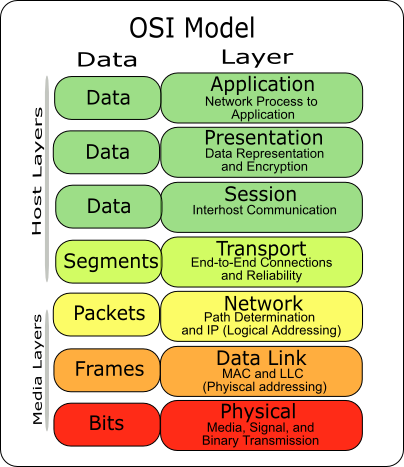
\includegraphics[width=.3\textwidth]{assets/osi/layers.png}
    \caption{The OSI Model Layers}\label{fig:osi_layers_intro}
\end{figure}
From chaos to order, the Open Systems Interconnection (OSI) model is a framework we use to understand how different networking protocols interact. Coincidentally (not so much), the Computer Networks course is structured around it.

\begin{table}[h]
    \centering
    \begin{tabular}{|c|c|c|}
        \hline
        \textbf{Layer} & \textbf{Function} & \textbf{Protocols} \\
        \hline
        Application & User interface & HTTP, FTP \\
        Presentation & Data translation & SSL/TLS \\
        Session & Session management & NetBIOS \\
        Transport & Data transfer & TCP, UDP \\
        Network & Routing & IP, ICMP \\
        Data Link & Node-to-node transfer & Ethernet \\
        Physical & Bit transmission & USB \\
        \hline
        \end{tabular}
    \caption{The Seven Layers of the OSI Model}\label{tab:osi_layers}
\end{table}

We will cover these layers by example in the next chapters, drilling down into layer-specific protocols and their intersections.


% Physical Layer
\chapter{Physical Layer}\label{sec:osi_physical}
\section{tl;dr}
The first layer of the OSI model is responsible for the physical transmission of data over a medium, with little to no concern for the content involved. It defines the hardware elements used in the communication process, such as cables, switches, and network interface cards (NICs).

\begin{noteblock}
    It might come across as a surprise, but routers are \textbf{not} part of the Physical Layer. The intuition as to why that is is that routers \textit{route}, hence they need to understand the content of the packets they are forwarding. This is a function of the Network Layer (Layer 3) in the OSI model.
\end{noteblock}

The Physical Layer is responsible for:
\begin{itemize}
    \item Converting bits to electrical, optical, or radio signals
    \item Defining voltage levels, timing, and physical data rates
    \item Specifying physical connectors and cable types
    \item Managing the physical topology of the network (which we'll be using Cisco Packet Tracer to visualize)
    \item Synchronizing transmission between devices
\end{itemize}

\newpage

\section{Transmission Media}
Different physical media carry the signals that transport our data across networks:

\subsection*{Guided Media}
Guided media confines signals to a specific path (literally "guided" along a cable or fiber). 

\subsubsection*{Twisted Pair Cable}
You probably know this one well, as you find it in most local area networks (LANs) and telephone systems. It consists of pairs of insulated copper wires twisted together to reduce electromagnetic interference.

\begin{figure}[h]
    \centering
    
\includegraphics[width=4cm]{assets/osi/physical/f-utp.png}
    \caption{F-UTP}\label{fig:twisted_pair}
\end{figure}

UTP (Unshielded Twisted Pair) is the most common type, but there are also shielded variants like STP (Shielded Twisted Pair) and F/UTP (Foiled Unshielded Twisted Pair).

\vspace{1em}

\subsubsection*{Coaxial Cable}
Usually used in cable television and broadband\footnote{Everything but dial-up.}.

\begin{figure}[h]
    \centering
    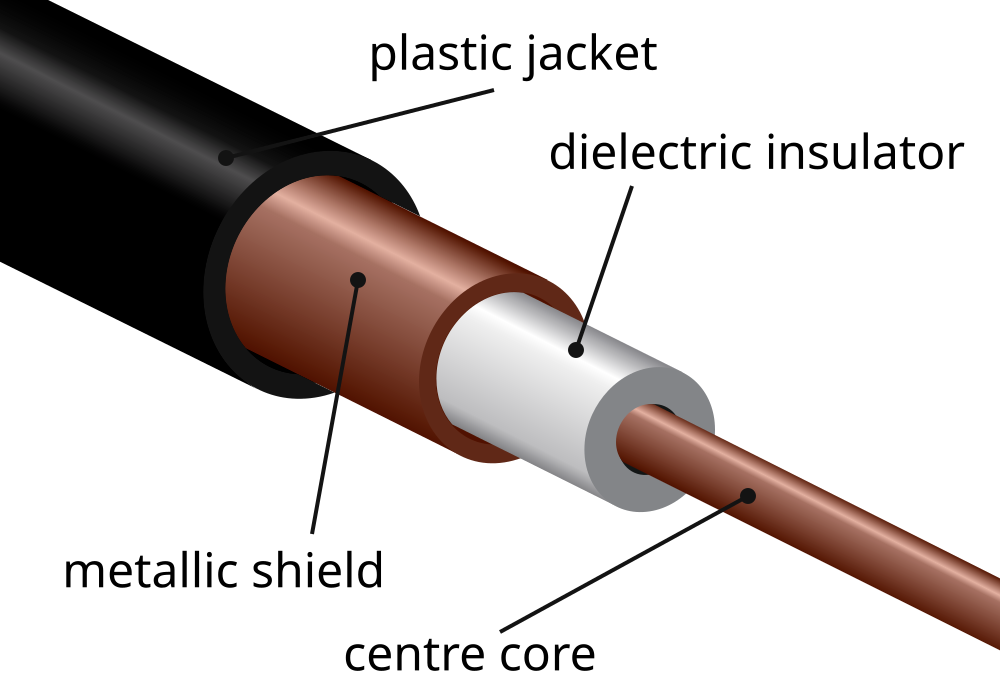
\includegraphics[width=4cm]{assets/osi/physical/coax.png}
    \caption{Coaxial cable structure}\label{fig:coaxial_cable}
\end{figure}

\begin{itemize}
    \item Common in cable TV networks and was used in early Ethernet implementations
    \item Offers better noise immunity than twisted pair with higher bandwidth capacity, which is why radio amateurs still use it
\end{itemize}

\vspace{1em}

\newpage
\subsubsection*{Fiber Optic Cable}
Uses light to transmit data, making it the fastest and most reliable medium available today.

\begin{itemize}
    \item Composed of a core, cladding, and protective outer layer
    \item Immune to electromagnetic interference
    \item Supports high bandwidths
\end{itemize}

\begin{figure}
    \centering
    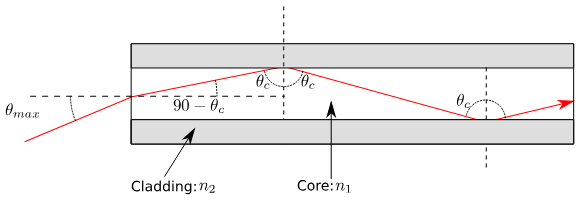
\includegraphics[width=.8\textwidth]{assets/osi/physical/fiber.png}
    \caption{Fiber optic cable structure}\label{fig:fiber_optic}
\end{figure}

\vspace{1em}

\subsection*{Wireless Transmission}
Ever wondered how signals travel through the air? Different types of electromagnetic waves are used for wireless communication, each with its own characteristics.

% assets/osi/physical/spectrum.png
\begin{figure}[h]
    \centering
    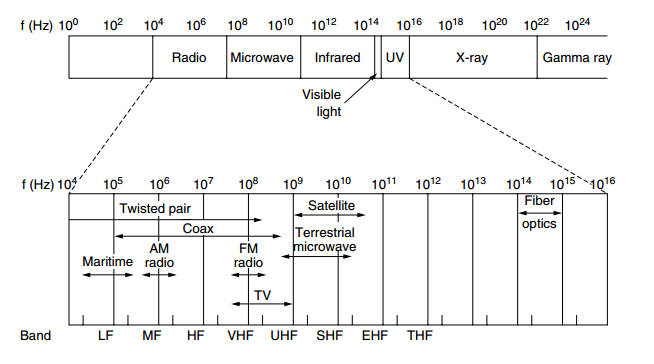
\includegraphics[width=.8\textwidth]{assets/osi/physical/spectrum.png}
    \caption{Electromagnetic spectrum showing different types of waves}\label{fig:em_spectrum}
\end{figure}

\subsubsection*{Radio Waves}
Radio waves are used for various wireless communication systems, including Wi-Fi, Bluetooth, and cellular networks. They can travel long distances (depending on wavelength) and penetrate through obstacles like walls.

\begin{noteblock}
    Fun fact! A lot of appliances like car remotes, thermostats and RC toys operate on the 433 MHz frequency band, which is a part of the radio spectrum. This is a perfect entry point if you'd like to hack your own devices or learn about radio communication.
\end{noteblock}

\subsubsection*{Microwaves}
Contrary to popular belief, microwaves are not just for cooking food. They are also used for point-to-point communication links, satellite communications, and some Wi-Fi networks. Microwaves have shorter wavelengths than radio waves, allowing them to carry more data, but faster attenuation\footnote{
    Attenuation: Reduction in signal strength as it travels through a medium, which can be caused by absorption, scattering, or reflection. 
    This is why we need repeaters/amplifiers!
} over distance.

\section{Standards and Specifications}
\subsection*{Ethernet Standards}
\begin{table}[h]
    \centering
    \begin{tabular}{|c|c|c|c|}
        \hline
        \textbf{Standard} & \textbf{Speed} & \textbf{Media} & \textbf{Distance} \\
        \hline
        10BASE-T & 10 Mbps & Cat3 UTP & 100m \\
        100BASE-TX & 100 Mbps & Cat5 UTP & 100m \\
        1000BASE-T & 1 Gbps & Cat5e UTP & 100m \\
        10GBASE-T & 10 Gbps & Cat6a UTP & 100m \\
        1000BASE-SX & 1 Gbps & Multi-mode fiber & 550m \\
        \hline
    \end{tabular}
    \caption{Common Ethernet Physical Layer Standards}\label{tab:ethernet_standards}
\end{table}

\subsection*{WiFi Standards}
\begin{itemize}
    \item 802.11a: 5 GHz, up to 54 Mbps
    \item 802.11b: 2.4 GHz, up to 11 Mbps
    \item 802.11g: 2.4 GHz, up to 54 Mbps
    \item 802.11n: 2.4/5 GHz, up to 600 Mbps
    \item 802.11ac: 5 GHz, up to 6.9 Gbps
    \item 802.11ax (WiFi 6): 2.4/5 GHz, up to 9.6 Gbps
\end{itemize}

\section{Signal Degradation}
Oh how we wish that signals could travel forever without losing strength! Unfortunately, they don't. As signals travel through a medium, they can degrade due to various factors like noise, interference, and attenuation.

This degradation can lead to errors in data transmission, which is why we need error detection and correction mechanisms in higher layers of the OSI model.

\subsection*{Shannon's Theorem and Channel Capacity}
Claude Shannon's groundbreaking work established the theoretical limits of data transmission over noisy channels. Shannon's theorem states that the maximum data rate (channel capacity) C of a noisy channel is given by:

\begin{equation}
C = B \log_2(1 + SNR)
\end{equation}

Where:
\begin{itemize}
    \item C = Channel capacity in bits per second (bps)
    \item B = Bandwidth in Hz
    \item SNR = Signal-to-Noise Ratio (linear, not in dB)
\end{itemize}

This formula tells us that even in the presence of noise, we can achieve error-free communication as long as our data rate doesn't exceed the channel capacity.

\subsection*{Nyquist's Theorem}
For noiseless channels, Harry Nyquist determined the maximum signaling rate. Nyquist's theorem states that the maximum data rate over a noiseless channel is:

\begin{equation}
C = 2B \log_2(V)
\end{equation}

Where:
\begin{itemize}
    \item C = Maximum data rate in bps
    \item B = Bandwidth in Hz
    \item V = Number of discrete signal levels
\end{itemize}

\begin{importantblock}
    Shannon's theorem considers noise and gives us the theoretical maximum for any channel, while Nyquist's theorem applies only to ideal, noiseless channels. In practice, Shannon's limit is more realistic since all real-world channels have noise.
\end{importantblock}

These theorems show us why we can't simply increase data rates indefinitely (which is something we really like doing when tackling complex problems) - physics imposes hard limits on information transmission!
\section{Data Exchange}
Think of it like this: you want to send a message to your friend across the room. You could:
\begin{itemize}
    \item Flash a light on and off (optical)
    \item Tap on the table (mechanical vibrations)
    \item Speak out loud (sound waves)
\end{itemize}

In networks, we do something similar but with electricity, light, or radio waves. The key insight is that we're just changing something physical that the receiver can detect - like voltage going up and down, light getting brighter and dimmer, or radio waves shifting frequency.

\begin{importantblock}
    The process of converting bits into signals is called \textbf{modulation}, and the reverse process is called \textbf{demodulation}.
\end{importantblock}



\subsection{The Reality Check}

Here's where it gets interesting. In an electrical engineer's ideal world, digital signals would look like perfect rectangles - instant jumps from 0 to 1. But physics says that the harsh reality is that a perfect one is impossible to achieve in practice\footnote{Source -- \href{https://en.wikipedia.org/wiki/Square_wave_(waveform)\#Characteristics_of_imperfect_square_waves}{https://en.wikipedia.org/wiki/Square\_wave\_(waveform)}}, due to the lack of infinite bandwidth required to create it. Real signals are always more sinusoidal, with smooth transitions between high and low states.

\begin{figure}[h]
    \centering
    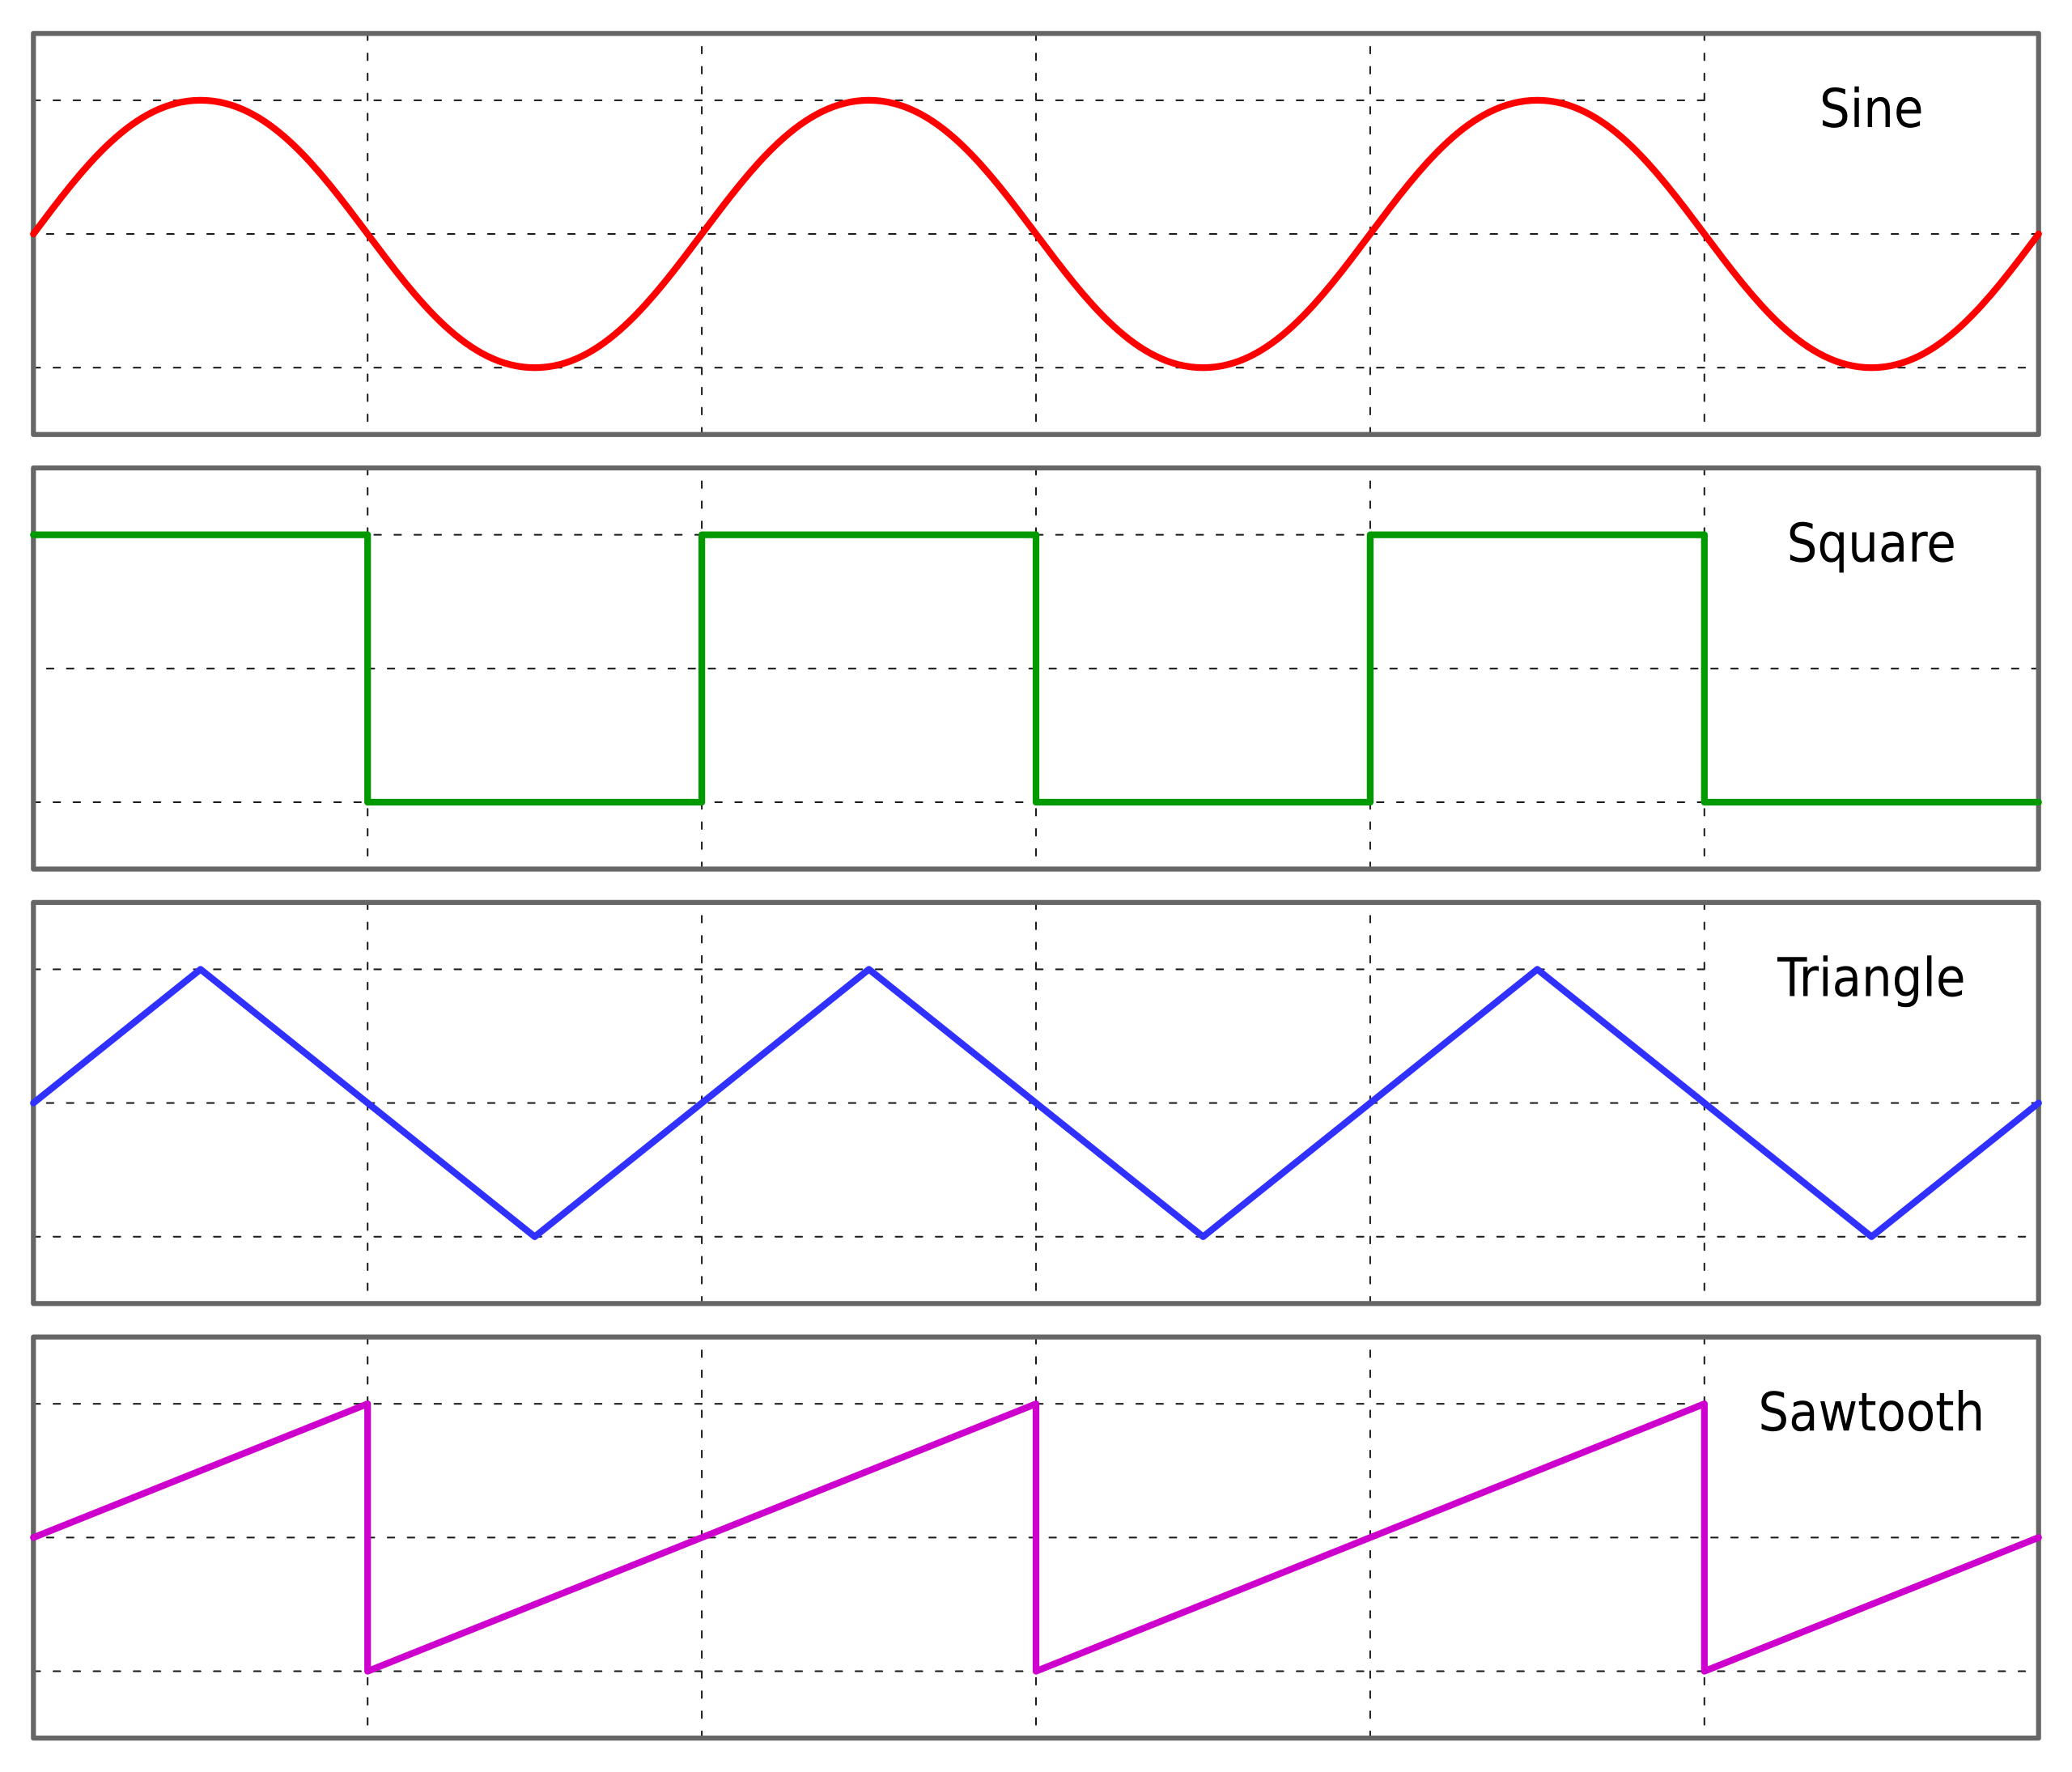
\includegraphics[width=.7\textwidth]{assets/osi/physical/waves.png}
    \caption{Theoretical waves}\label{fig:theoretical_waves}
\end{figure}

In practice, we use analog signals to transmit digital information. These analog signals are continuous and can take any value within a range. At the receiver, we need to convert these analog signals back to discrete digital values (\texttt{1} or \texttt{0}) through a process called \textbf{sampling and quantization}. The receiver samples the analog signal at specific time intervals and uses threshold levels to determine whether each sample represents a \texttt{1} or \texttt{0}.

Let's look at a simple example of a 1-bit ADC (Analog to Digital Converter) that converts a voltage level into a bit value:

% assets/osi/physical/adc_plot.png
\begin{figure}[h]
    \centering
    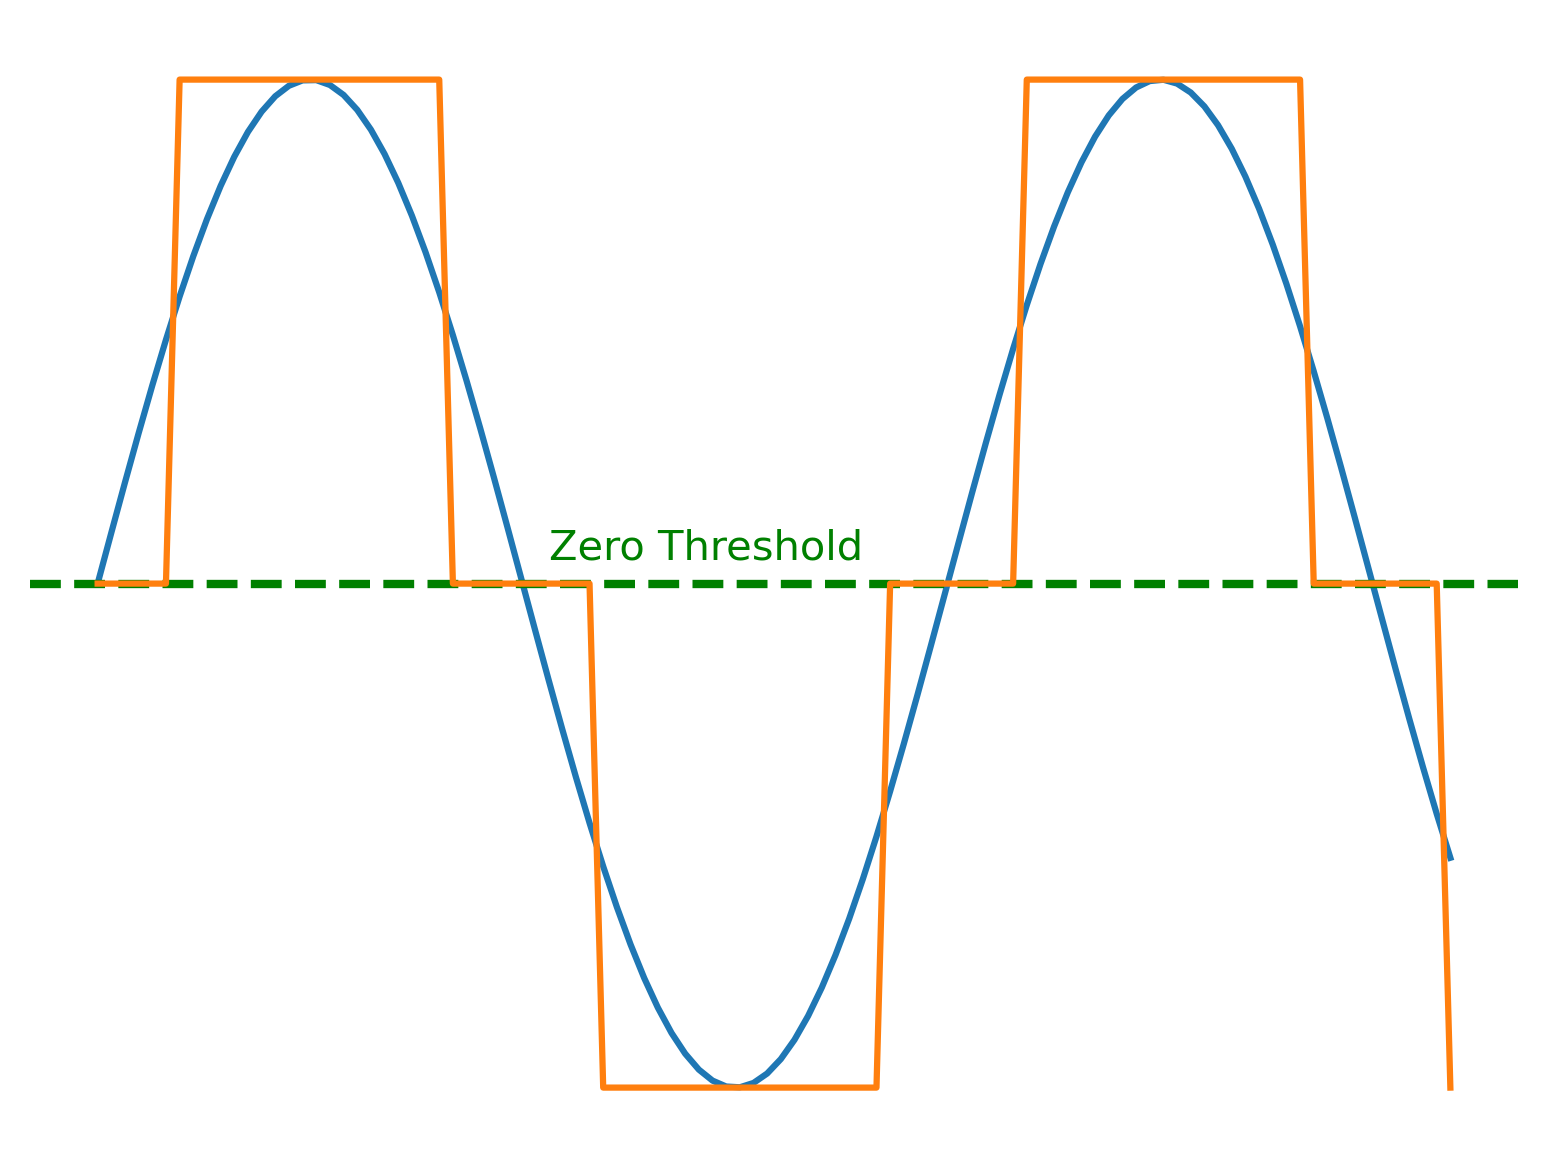
\includegraphics[width=.5\textwidth]{assets/osi/physical/adc_plot.png}
    \caption{Example of a 1-bit ADC converting voltage levels to bits}\label{fig:adc_plot}
\end{figure}

However, as you can probably guess, there are infinite ways for us to interpret this graph. It could correspond to \texttt{1010} or \texttt{1111000011110000} and so on. 
This is where clock signals come into play, which help us determine when to sample the signal and how to interpret it.

\subsection*{Let's talk timing $\star$}
Clocks or timing signals are present in all hardware communication. 

The idea is to ensure that both sender and receiver are synchronized in their understanding of when bits are being sent and received. 

As an analogy, think of a dance where both partners need to be in sync to perform the moves correctly. If one partner is out of sync, the dance will look awkward and may not work at all.


There are two main types of synchronization:
\begin{itemize}
    \item Both sender and receiver share a common clock signal (Figure~\ref{fig:clock_sync}) - Synchronous 
    \item Sender and receiver do not share a common clock, but use start and stop bits to indicate the beginning and end of a data frame - Asynchronous
\end{itemize}

\begin{figure}[h]
    \centering
    \begin{tikzpicture}
        % Clock signal
        \draw[thick] (0,2) -- (0.5,2) -- (0.5,3) -- (1,3) -- (1,2) -- (1.5,2) -- (1.5,3) -- (2,3) -- (2,2) -- (2.5,2) -- (2.5,3) -- (3,3) -- (3,2) -- (3.5,2) -- (3.5,3) -- (4,3) -- (4,2) -- (4.5,2);
        \node at (-0.5,2.5) {Clock};
        
        % Data signal
        \draw[thick] (0,0.5) -- (1,0.5) -- (1,1.5) -- (2,1.5) -- (2,0.5) -- (3.5,0.5) -- (3.5,1.5) -- (4.5,1.5);
        \node at (-0.5,1) {Data};
        
        % Sampling points
        \foreach \x in {0.5,1.5,2.5,3.5}
            \draw[red,thick] (\x,0.2) -- (\x,1.8);
        
        % Bit values
        \node at (0.5,0) {0};
        \node at (1.5,0) {1};
        \node at (2.5,0) {0};
        \node at (3.5,0) {1};
        
        % Labels
        \node at (2.25,-0.5) {Bit sampling occurs on clock transitions};
    \end{tikzpicture}
    \caption{Example rising edge clock synchronization}\label{fig:clock_sync}
\end{figure}

\vfill
In asynchronous serial\footnote{
    Serial - \textit{one after another} - communication, data is sent one bit at a time over a single channel. This is in contrast to parallel communication. More on that in the Operating Systems course.
} communication, data is organized into discrete blocks called code words of fixed length - usually bytes or ASCII characters (\texttt{char}s are $2^8 = 256$ bits, i.e. a byte). Each code word is framed by:

\begin{figure}[h]
    \centering
    \input{assets/diagrams/physical.latex}
    \caption{Async serial frame structure}\label{fig:async_frame}
\end{figure}

This approach, specifically in the form that we refer to in the figure, is \textbf{character-oriented}.
\vfill
\section{Modulation and Encoding}
As mentioned earlier, modulation is the process of converting digital data into analog signals for transmission over a physical medium.

\begin{figure}[h]
    \centering
    
\includegraphics[width=\textwidth]{assets/osi/physical/signals/modulation.png}
    \caption{Modulation techniques}\label{fig:modulation_techniques}
\end{figure}

\subsection{The basics}
We'll start with something most people are familiar with, as it is used in consumer radios! The ones you listen to in your car or at home.

Amplitude Modulation (AM) and Frequency Modulation (FM) are two very common modulations used in radio broadcasting, where we are used to hearing music and news. We are used to tuning our radios to a specific frequency ($\approx$ 80-100 MHz for FM and usually way lower for AM) to listen to our favorite stations.

There's also Phase Modulation (PM), where the phase of the carrier wave is varied according to the input signal.
\begin{figure}[h]
    \centering
    \begin{tikzpicture}[scale=0.8]
        % AM Signal
        \begin{scope}[shift={(0,0)}]
            \draw[->] (0,0) -- (4.5,0) node[right] {$t$};
            \draw[->] (0,-1.5) -- (0,1.5) node[above] {$A(t)$};
            \draw[domain=0:4,samples=200,thick,blue] plot (\x,{(1+0.5*sin(2*\x r))*sin(20*\x r)});
        \end{scope}
        
        % FM Signal
        \begin{scope}[shift={(6,0)}]
            \draw[->] (0,0) -- (4.5,0) node[right] {$t$};
            \draw[->] (0,-1.5) -- (0,1.5) node[above] {$A(t)$};
            \draw[domain=0:4,samples=200,thick,red] plot (\x,{sin(20*\x r + 2*sin(2*\x r))});
        \end{scope}
        
        % PM Signal
        \begin{scope}[shift={(12,0)}]
            \draw[->] (0,0) -- (4.5,0) node[right] {$t$};
            \draw[->] (0,-1.5) -- (0,1.5) node[above] {$A(t)$};
            \draw[domain=0:4,samples=200,thick,green!50!black] plot (\x,{sin(20*\x r + 0.5*sin(2*\x r))});
        \end{scope}
    \end{tikzpicture}
    \caption{Graphical representation of \textcolor{blue}{AM}, \textcolor{red}{FM}, and \textcolor{green!50!black}{PM} signals.}\label{fig:modulation_math}
\end{figure}


But wait, we have only heard voices and music, not bits! How does that work?

The answer lies in \textbf{digital modulation}! While AM and FM were originally designed for analog voice transmission, the same radio frequencies can carry digital data using techniques like DMR, WSPR, and many, many more.
These digital protocols use discrete changes in amplitude, frequency, or phase to represent bits.

For example, in WSPR, a \texttt{1} might be represented by a short burst of a specific frequency, while a \texttt{0} might be represented by silence or a different frequency - this is called \textbf{frequency-shift keying (FSK)}.


\begin{figure}[h]
    \centering
    \begin{subfigure}[b]{0.2\textwidth}
        \centering
        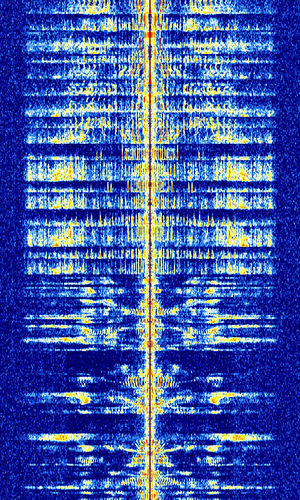
\includegraphics[width=\textwidth]{assets/osi/physical/signals/am_voice.png}
        \caption{AM Voice Signal}
        \label{fig:am_voice}
    \end{subfigure}
    \hspace{1em}
    \begin{subfigure}[b]{0.2\textwidth}
        \centering
        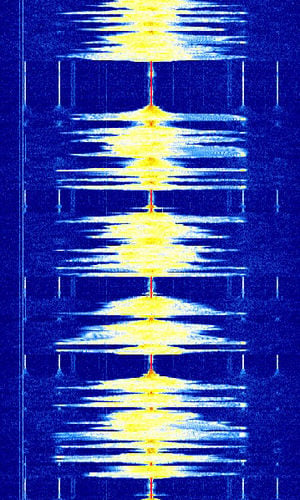
\includegraphics[width=\textwidth]{assets/osi/physical/signals/fm_voice.png}
        \caption{FM Voice Signal}
        \label{fig:fm_voice}
    \end{subfigure}
    \hspace{1em}
    \begin{subfigure}[b]{0.2\textwidth}
        \centering
        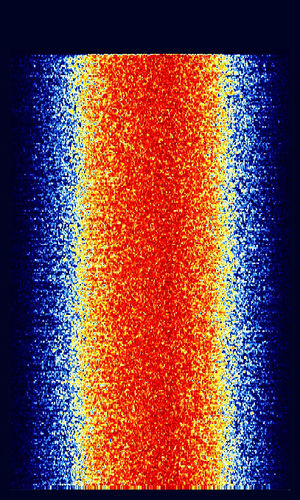
\includegraphics[width=\textwidth]{assets/osi/physical/signals/dmr.png}
        \caption{DMR Digital Signal}
        \label{fig:dmr_digital}
    \end{subfigure}
    \hspace{1em}
    \begin{subfigure}[b]{0.2\textwidth}
        \centering
        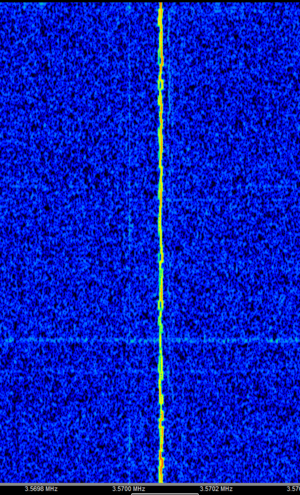
\includegraphics[width=\textwidth]{assets/osi/physical/signals/wspr.png}
        \caption{WSPR Digital Protocol}
        \label{fig:wspr_digital}
    \end{subfigure}
    
    \caption{Comparison of analog voice signals (a, b) vs digital signals (c, d) in the radio spectrum. Sourced from sigidwiki.com}
    \label{fig:analog_vs_digital_signals}
\end{figure}

\newpage
For digital data, modulation becomes synonymous with \textbf{keying}, where we use changes in the signal to represent bits.

\begin{itemize}
    \item Amplitude Shift Keying (ASK) -  A higher amplitude might represent a \texttt{1}, while a lower amplitude represents a \texttt{0}.
    \item Frequency Shift Keying (FSK) - Different frequencies represent different bits.
    \item Phase Shift Keying (PSK) - A phase shift might represent a \texttt{1}, while no shift represents a \texttt{0}.
\end{itemize}
\begin{figure}[h]
    \centering
    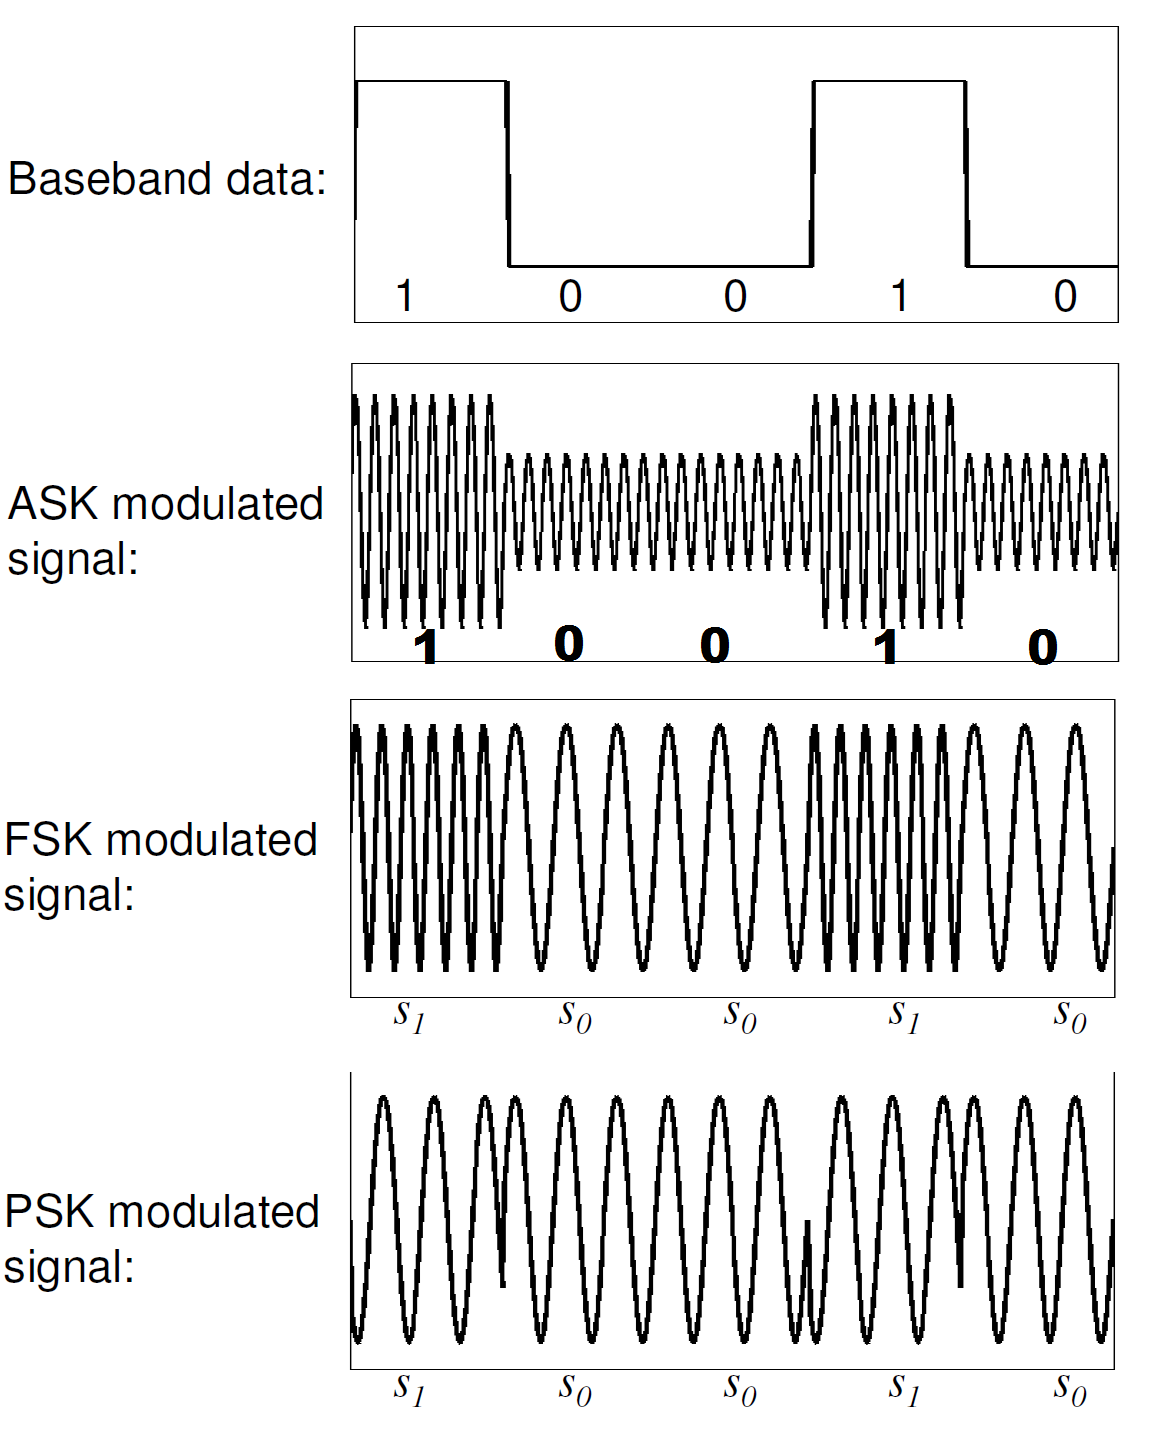
\includegraphics[width=0.45\textwidth]{assets/osi/physical/signals/sk.png}
    \caption{Keying techniques: ASK, FSK, PSK}\label{fig:keying_techniques}
\end{figure}

\subsection{Quadrature Amplitude Modulation (QAM)}
What if we could send multiple bits at once? That's where QAM comes in, which is a combination of both amplitude and phase modulation.

`Quadrature' just means we're using two waves that are perfectly out of sync - 90 degrees out of phase, to be exact (quad = four, so in a circle $\frac{360}{4} = 90$).

\subsubsection{Complex Numbers and QAM $\star$}
To completely understand QAM, we will need to quickly refresh our knowledge of complex numbers. If you are not familiar with them, I recommend reading the \href{https://en.wikipedia.org/wiki/Complex_number}{Wikipedia article}. 

QAM transmits data using two independent carrier waves at the same frequency but shifted 90 degrees apart in phase - called `in-phase' ($I$) and `quadrature' ($Q$) components. This orthogonal\footnote{
    Remember orthogonality! It's a cheat code in signal processing! It means the two signals don't interfere with each other and can be separated at the receiver.
} relationship means the two signals don't interfere with each other and can be separated at the receiver.

Complex numbers provide an elegant mathematical framework for this because:
\begin{itemize}
    \item The real part represents the in-phase ($I$) component
    \item The imaginary part represents the quadrature ($Q$) component  
    \item A 90-degree phase shift is equivalent to multiplication by $i$ (since $e^{i\pi/2} = i$)
    \item Both amplitude and phase information are present in a single complex number $z = $I$ + iQ$
\end{itemize}

\begin{figure}[h]
    \centering
    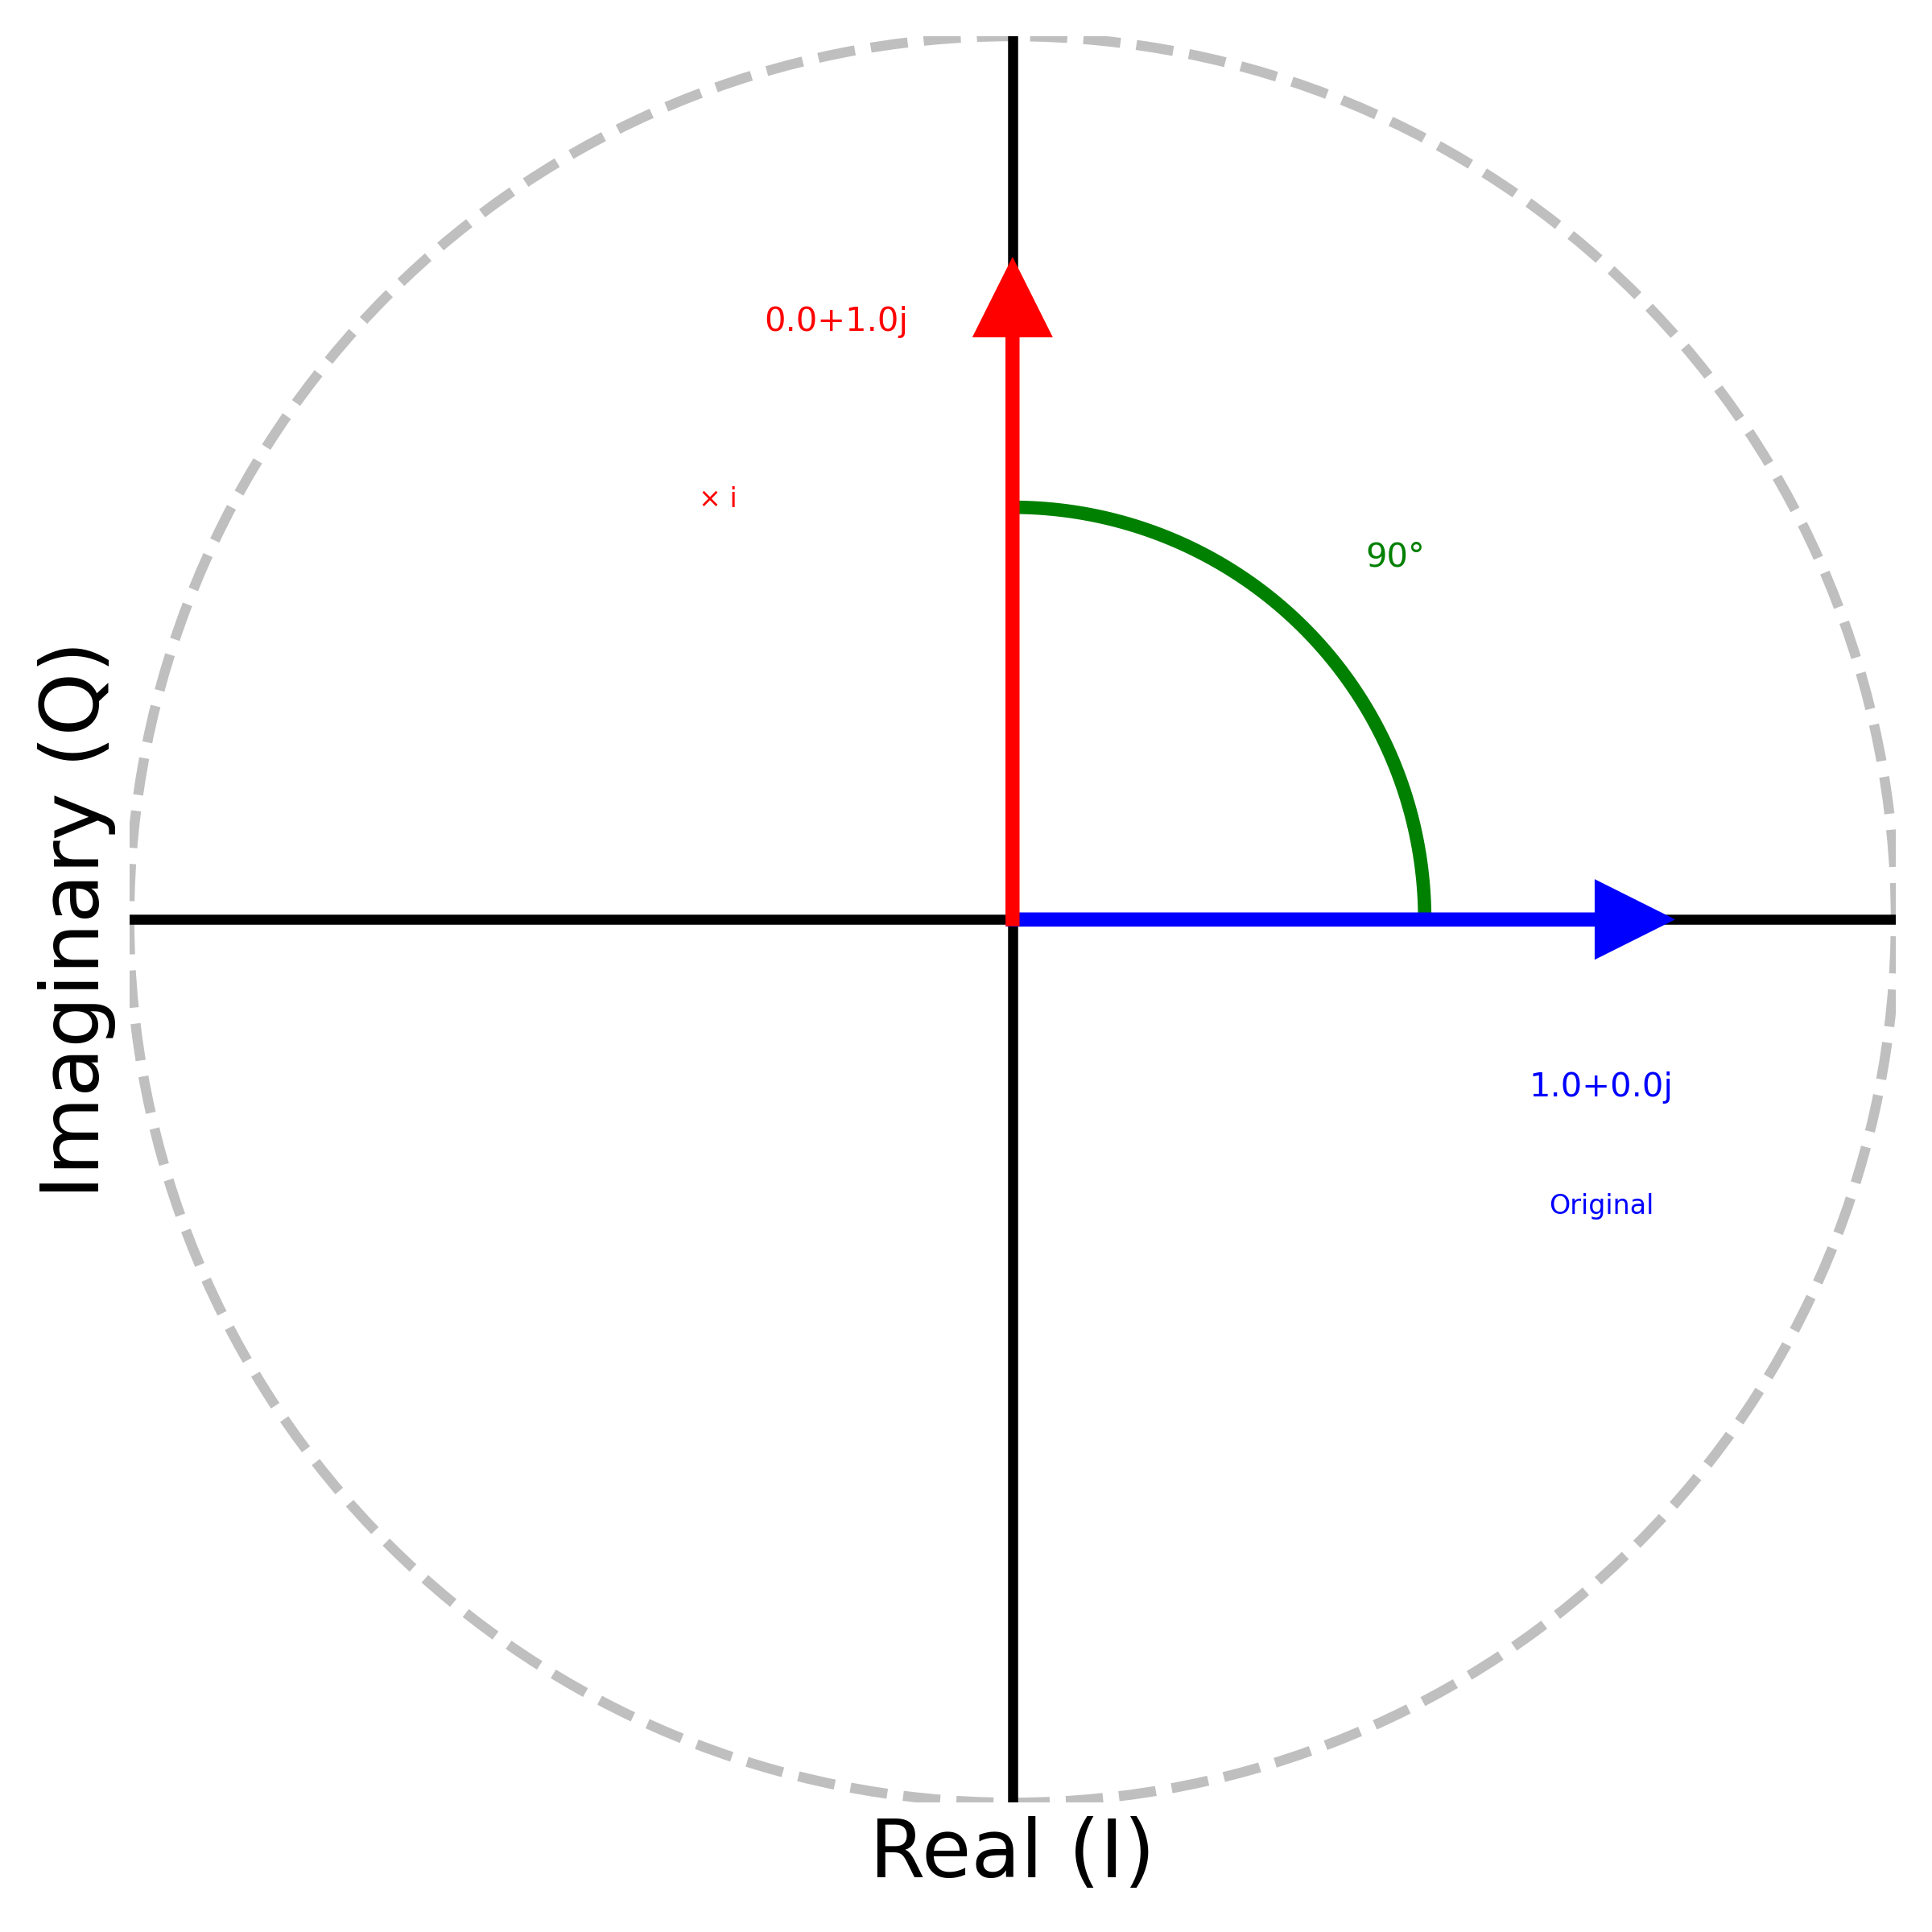
\includegraphics[width=0.5\textwidth]{assets/diagrams/iq.png}
\end{figure}

This is why we call it "Quadrature" - it literally refers to the four quadrants of this complex plane, where signals can point in any direction to encode different bit combinations.

\subsubsection{What does the number mean?}
When working with QAM, we will often see terms like 16-QAM, 64-QAM, etc. These numbers refer to the number of distinct symbols that can be transmitted. For example:
\begin{itemize}
    \item 16-QAM can transmit 16 different symbols, each representing 4 bits
    \item 64-QAM can transmit 64 different symbols, each representing 6 bits
    \item 256-QAM can transmit 256 different symbols, each representing 8 bits
\end{itemize}

You may notice the pattern in the above examples - the number of bits per symbol is given by $\log_2(N)$, where $N$ is the number of symbols.

This will immediately make sense in the next section.
\subsection{Constellation Diagrams}
A constellation diagram is a graphical representation of digital modulation schemes. Each point in the diagram represents a unique symbol that can be transmitted, with its position determined by the signal's characteristics. That's nerdspeak for points on a graph.

\begin{figure}[h]
    \centering
    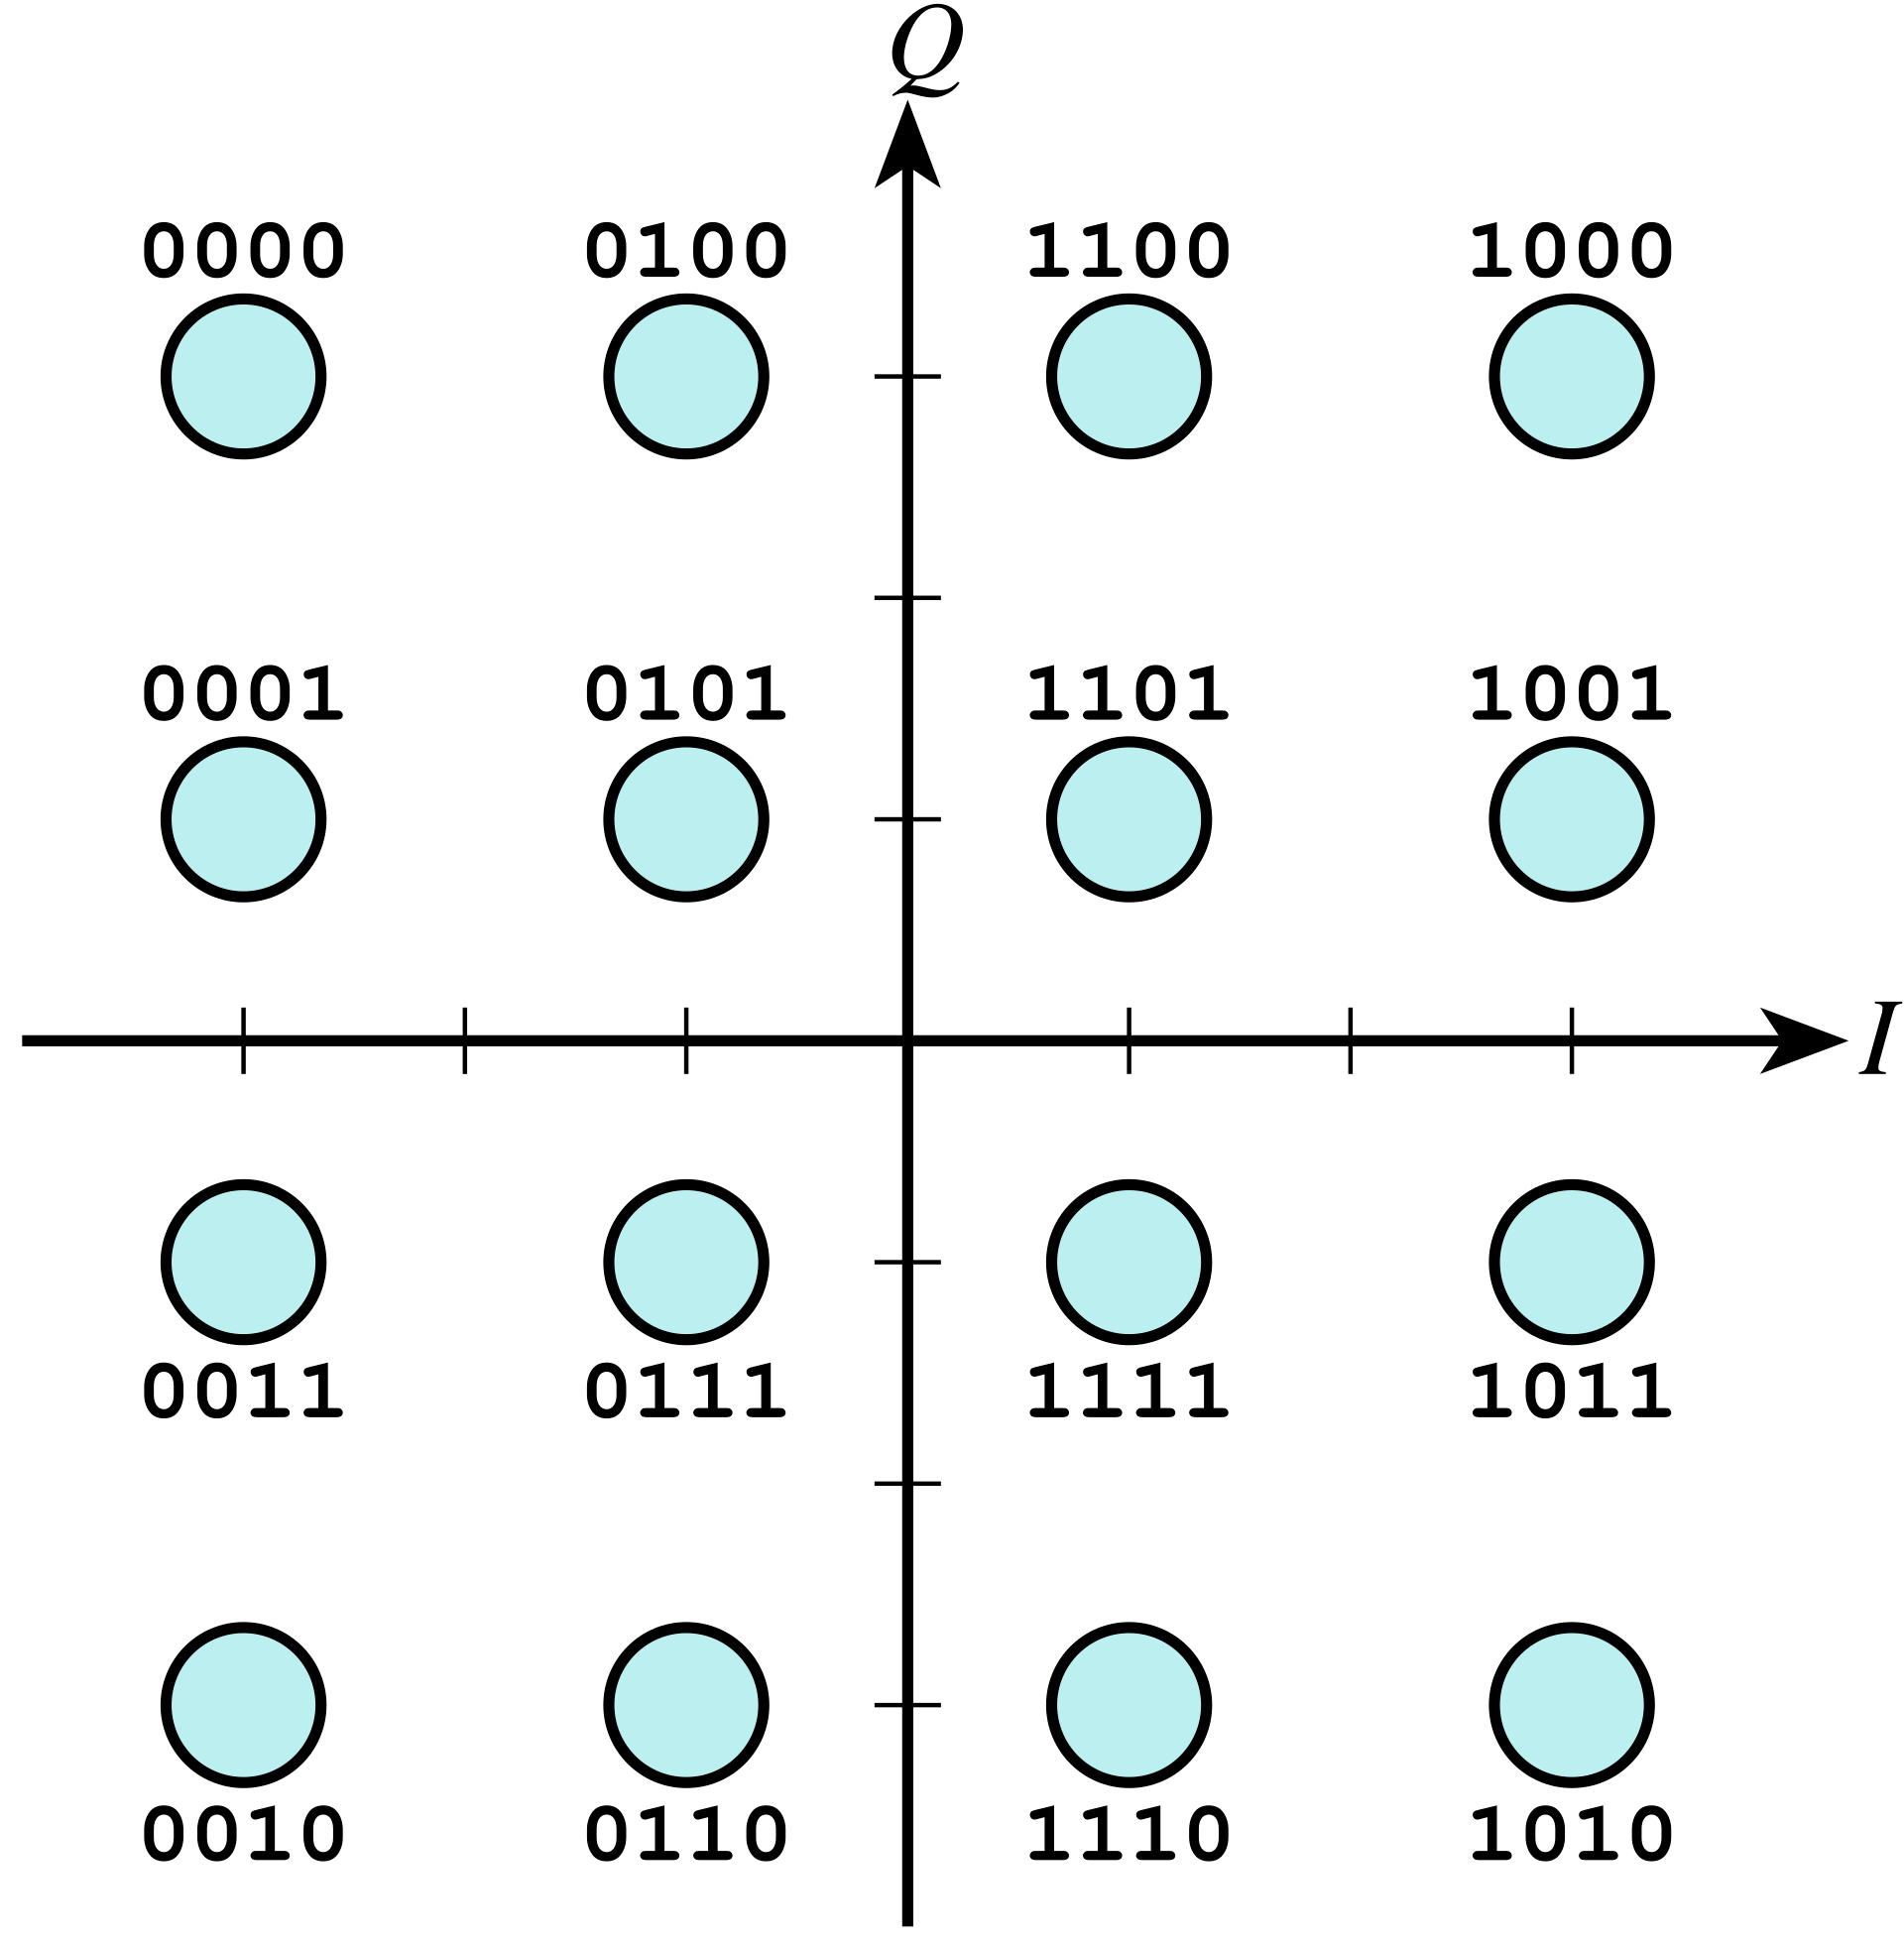
\includegraphics[width=0.5\textwidth]{assets/osi/physical/signals/qam.png}
    \caption{Example of a 16-QAM \textbf{cartesian} constellation diagram}\label{fig:qam_constellation}
\end{figure}


For QAM, the position is determined by the in-phase ($I$) and quadrature ($Q$) components (x, y coordinates). For other modulation schemes:
\begin{itemize}
    \item In PSK, points are arranged in a circle, with phase determining the angular position
    \item In ASK, points are arranged on a line, with amplitude determining the position
\end{itemize}

\begin{importantblock}
    You can probably see that ASK+PSK is QAM, since, by definition, it combines both amplitude and phase modulation.
\end{importantblock}

In any constellation diagram, each point represents a unique combination of signal parameters. The distance between points determines the minimum distance between symbols, which affects the error rate in transmission. The more points we have, the more bits we can transmit per symbol, but the closer they are together, the easier it is to confuse them at the receiver.

There are different ways to visualize these diagrams, for example, when treating ASK+PSK (component-wise, instead as a single complex number), we can plot the amplitude and phase separately as concentric circles with points scattered accross their respective circumferences. This is called a \textbf{polar constellation diagram}.

Let's look at an example of a 4-QAM (ASK+PSK) constellation diagram.
\begin{figure}[h]
    \centering
    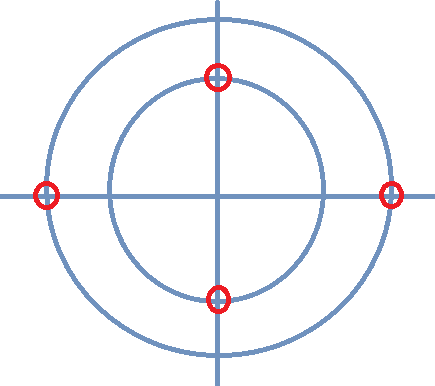
\includegraphics[width=0.5\textwidth]{assets/osi/physical/signals/ask+psk.png}
    \caption{Example of a 4-QAM \textbf{polar constellation diagram}}\label{fig:ask_psk_constellation}
\end{figure}

Now, say we want to encode the binary string \texttt{00101101}. We can map it to the 4-QAM constellation diagram as follows:

\begin{itemize}
    \item \texttt{00} maps to the first point on the left of outer circle
    \item \texttt{10} maps to the second point on the top of inner circle
    \item \texttt{11} maps to the third point on the right of outer circle
    \item \texttt{01} maps to the fourth point on the bottom of inner circle
\end{itemize}

Resulting in the following mapping:
\begin{figure}[h]
    \centering
    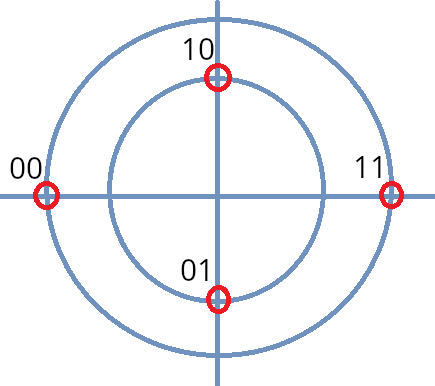
\includegraphics[width=0.5\textwidth]{assets/osi/physical/signals/ask+psk_filled.png}
    \caption{Example of a 4-QAM constellation diagram with bits mapped to points}\
    \label{fig:ask_psk_filled_constellation}
\end{figure}

Again, this mapping is arbitrary, and we can choose any mapping we want, as long as the receiver knows how to interpret it (which, hypothetically, it always does).

Since we have both amplitude and phase information for each constellation point, we can plot the actual time-domain waveforms that correspond to each symbol - showing how the signal actually looks during transmission!

Let's do so for this example.

\subsubsection{Time-Domain Waveforms}
Each constellation point can be expressed as a complex number with amplitude $A$ and phase $\phi$:
$$s(t) = A \cos(2\pi f_c t + \phi)$$

where $f_c$ is the carrier frequency. For our 4-QAM example with bit string \texttt{00101101}, the complete transmitted signal looks like:

\begin{figure}[h]
    \centering
    \begin{tikzpicture}[scale=1]
        % Main axes
        \draw[->] (0,0) -- (13,0) node[right] {Time};
        \draw[->] (0,-2) -- (0,2) node[above] {Amplitude};
        
        % Symbol boundaries (vertical dashed lines)
        \foreach \x in {3,6,9,12} {
            \draw[dashed, gray] (\x,-2) -- (\x,2);
        }
        
        % Symbol period labels
        \node[below] at (1.5,-2.3) {\texttt{00}};
        \node[below] at (4.5,-2.3) {\texttt{10}};
        \node[below] at (7.5,-2.3) {\texttt{11}};
        \node[below] at (10.5,-2.3) {\texttt{01}};
        
        % Symbol period markers
        \node[below] at (1.5,-2.6) {$T_s$};
        \node[below] at (4.5,-2.6) {$T_s$};
        \node[below] at (7.5,-2.6) {$T_s$};
        \node[below] at (10.5,-2.6) {$T_s$};
        
        % Complete waveform
        % Symbol 1: 00 (High amp, 180° phase) - inverted high amplitude cosine
        \draw[domain=0:3,samples=150,thick,blue] plot (\x,{1.5*cos(8*\x r + 180)});
        
        % Symbol 2: 10 (Low amp, 90° phase) - low amplitude sine  
        \draw[domain=3:6,samples=150,thick,red] plot (\x,{0.8*cos(8*\x r + 90)});
        
        % Symbol 3: 11 (High amp, 0° phase) - normal high amplitude cosine
        \draw[domain=6:9,samples=150,thick,green!60!black] plot (\x,{1.5*cos(8*\x r)});
        
        % Symbol 4: 01 (Low amp, 270° phase) - low amplitude negative sine
        \draw[domain=9:12,samples=150,thick,orange] plot (\x,{0.8*cos(8*\x r + 270)});
        
        % Amplitude level indicators
        \draw[dotted, gray] (0,1.5) -- (12.5,1.5) node[right] {\small High};
        \draw[dotted, gray] (0,0.8) -- (12.5,0.8) node[right] {\small Low};
        \draw[dotted, gray] (0,-0.8) -- (12.5,-0.8);
        \draw[dotted, gray] (0,-1.5) -- (12.5,-1.5);
        
        % Time axis labels
        \node[below] at (0,-0.2) {0};
        \node[below] at (3,-0.2) {$T_s$};
        \node[below] at (6,-0.2) {$2T_s$};
        \node[below] at (9,-0.2) {$3T_s$};
        \node[below] at (12,-0.2) {$4T_s$};
    \end{tikzpicture}
    \caption{Complete time-domain signal for bit string \texttt{00101101} using 4-QAM modulation. Each symbol period $T_s$ contains one constellation point with its specific amplitude and phase.}
    \label{fig:qam_complete_waveform}
\end{figure}

\begin{tipblock}
    In practice, these individual symbol waveforms are concatenated to form the complete transmitted signal. The receiver uses matched filtering and decision algorithms to determine which constellation point was transmitted by analyzing the received waveform during each symbol period.
\end{tipblock}
\section{Multiplexing}
\label{sec:multiplexing}
Okay, we've covered how data gets transmitted over a medium and how we can modulate signals to represent our data. That's cool! Unfortunately, with the busy lives we lead, we need lots of data - fast! So, how do we cram all this data into our limited bandwidth? Enter multiplexing!

Multiplexing is the technique of combining multiple signals into one signal over a shared medium. This allows us to make the most out of our available bandwidth by sending multiple data streams simultaneously.

\subsection{Time Division Multiplexing (TDM)}
\label{subsec:tdm}
Time Division Multiplexing (TDM) is a method where multiple signals share the same transmission medium by dividing the time into slots. Each signal gets its own time slot to transmit its data, and the slots are allocated in a round-robin fashion. This way, each signal gets a chance to transmit without interfering with others.

TODO

\subsection{Frequency Division Multiplexing (FDM)}
\label{subsec:fdm}
Frequency Division Multiplexing (FDM) is another technique where multiple signals are transmitted simultaneously over different frequency bands. Each signal occupies a unique frequency range, allowing them to coexist without interference. This
is commonly used in radio and television broadcasting, where different channels are assigned specific frequency bands.


TODO

\subsection{Code Division Multiple Access (CDMA)}
\label{subsec:cdma}
Code Division Multiple Access (CDMA) is a more advanced multiplexing technique that allows multiple signals to share the same frequency band simultaneously. Each signal is assigned a unique code, which is used to modulate the signal. At the receiver, the unique code is used to demodulate the signal and extract the original data. This technique is widely used in mobile communication systems, allowing multiple users to share the same frequency band without interference.

TODO: Chip codes and such
% ===== APPENDICES =====
\appendix


% ===== BACK MATTER =====
\backmatter
\listoffigures
\listoftables
\chapter*{Contributions}\label{sec:contributions}

\subsection*{@confestim - 28/07/25}
asdfds
\url{https://github.com/confestim/CN-Reader/pull/8}

\end{document}